\documentclass[10pt]{beamer}

% \usetheme{Montpellier}

\usepackage[T1]{fontenc}
\usepackage[utf8]{inputenc}  
\usefonttheme{professionalfonts}

\setbeamersize{text margin left=30pt, text margin right=30pt}

\setbeamercolor{section in head/foot}{fg=blue}

\title{Présentation projet final PP-GPU}
\author{Matthieu PETIT \\ Djemsay MORVAN \\ Ulysse CAROMEL}
\setbeamertemplate{section in toc}[sections numbered]
\setbeamertemplate{navigation symbols}{}
\setbeamertemplate{itemize items}[square]

\begin{document}
\begin{frame}
    
\includegraphics[width=0.2\textwidth]{Images/univ-rennes1.png}
    \rule{\linewidth}{0.3mm} \\[0.4cm]
    \titlepage
    \rule{\linewidth}{0.3mm} \\[0.4cm]
\end{frame}

\begin{frame}
    \frametitle[Table des matières]{Table des matières}
    \tableofcontents
\end{frame}

\section{Les différentes méthodes d'intégration}

\begin{frame}
    \frametitle{Méthodes d'intégration}  
    \tableofcontents[currentsection]  
\end{frame}

\subsection{Méthode de Simpson}


\begin{frame}
    {\fontsize{4}{5}\selectfont Texte en police très petite}

    \frametitle{Méthode de Simpson}

    \begin{itemize}
        \item Division de l'intervalle $[a, b]$ en sous-intervalles de largeur égale $h = \frac{b - a}{n}$, $n$ étant pair.
        
        \item Approximation sur chaque sous-intervalle $[x_i, x_{i+2}]$ :
            \[
            \int_{x_i}^{x_{i+2}} f(x) \,dx \approx \frac{h}{3} \left[ f(x_i) + 4f(x_{i+1}) + f(x_{i+2}) \right]
            \]
        
        \item Estimation finale de l'intégrale :
            \begin{align*}
                \int_{a}^{b} f(x) \,dx \approx \frac{h}{3} \Big [ f(a) + 4f(x_1) + 2f(x_2) &+ \ldots + 2f(x_{n-2})  \\
                &+ 4f(x_{n-1}) + f(b) \Big ]
            \end{align*}
    \end{itemize}
    
\end{frame}


\subsection{Méthode de Gauss 2D}
\begin{frame}
    \frametitle{Quadrature Gaussienne 2D}
    \footnotesize
    \begin{itemize}
        \item Estimation numérique de l'intégrale d'une fonction $f(x, y)$ sur une région bidimensionnelle définie par $a \leq x \leq b$ et $c \leq y \leq d$.
        
        \item Utilise un ensemble de points et de poids associés pour approximer l'intégrale.
        
        \item Formule générale :
            \begin{align*}
            \iint_{R} f(x, y) \,dx\,dy \approx \sum_{i=1}^{n} \sum_{j=1}^{m} w_{ij} \cdot f(x_i, y_j)
            \end{align*}
        
        \item Formule spécifique pour un quadrilatère :
            \begin{align*}
            \iint_{R} f(x, y) \,dx\,dy \approx & \sum_{i=1}^{n} \sum_{j=1}^{m} w_{ij} \cdot f\Bigg(\frac{1}{2}(1 + \xi_i)x\\
             &+ \frac{1}{2}(1 - \xi_i)y, \frac{1}{2}(1 + \eta_j)x + \frac{1}{2}(1 - \eta_j)y\Bigg)
            \end{align*}
        
        \item Offre une précision supérieure à la quadrature de Gauss unidimensionnelle.
    \end{itemize}
\end{frame}

\subsection{Méthode de Runge-Kutta}
\begin{frame}
    \frametitle{Méthode de Runge-Kutta (RK4) pour les EDO}
    \small
    \begin{itemize}
        \item Technique numérique pour résoudre des équations différentielles ordinaires (EDO).
        
        \item Méthode de Runge-Kutta d'ordre 4 (RK4) : équilibre entre précision et complexité.
        
        \item Forme générale d'une EDO du premier ordre :
            \[
            \frac{dy}{dt} = f(t, y)
            \]
        
        \item Étapes de la méthode RK4 :
            \begin{align*}
            k_1 &= h \cdot f(t_n, y_n) \\
            k_2 &= h \cdot f(t_n + \frac{h}{2}, y_n + \frac{k_1}{2}) \\
            k_3 &= h \cdot f(t_n + \frac{h}{2}, y_n + \frac{k_2}{2}) \\
            k_4 &= h \cdot f(t_n + h, y_n + k_3)
            \end{align*}
        
        \item Mise à jour de la solution à chaque pas :
            \begin{align*}
             y_{n+1} = y_n + \frac{1}{6}(k_1 + 2k_2 + 2k_3 + k_4)
            \end{align*}
        
        \item Offre une meilleure précision que des méthodes de pas fixe plus simples, largement utilisée pour sa robustesse et polyvalence.
    \end{itemize}
\end{frame}

\subsection{Méthode de Monte-Carlo}
\begin{frame}
    \frametitle{Méthode de Monte Carlo pour l'intégration}
    \small
    \begin{itemize}
        \item Utilisée pour estimer numériquement des intégrales complexes, notamment dans des espaces multidimensionnels.
        
        \item Fondée sur des principes probabilistes, associant le hasard à des calculs numériques.
        
        \item Estimation d'une valeur en utilisant des échantillons aléatoires dans un domaine donné.
        
        \item Génération de points aléatoires dans le domaine $D$.
        
        \item Évaluation de la fonction $f(x, y)$ pour chaque point généré.
        
        \item Calcul de la moyenne pondérée des valeurs de $f(x, y)$ pour les points générés, multipliée par la mesure de $D$.
    \end{itemize}

    Formule d'estimation de Monte Carlo pour l'intégrale :
    $$I \approx A \cdot \frac{1}{N} \sum_{i=1}^{N} f(x_i, y_i)$$

    Avantages : Flexibilité, capacité à traiter des problèmes complexes en dimensions élevées. Précision dépend du nombre de points aléatoires générés.

\end{frame}

\subsection{Comparaison des méthodes}
% \begin{frame}
%     \small
%     \frametitle{Comparaison des Méthodes Numériques}
%     \begin{itemize}
%         \item \textbf{Quadrature Gaussienne 2D (Gauss 2D):}
%             \begin{itemize}
%                 \item \textbf{Avantages :} Précision élevée, adaptée aux intégrales sur des domaines bidimensionnels complexes.
%                 \item \textbf{Inconvénients :} Nécessite la connaissance de la fonction à intégrer, plus de calculs.
%             \end{itemize}

%         \item \textbf{Méthode de Runge-Kutta (RK4) pour les EDO :}
%             \begin{itemize}
%                 \item \textbf{Avantages :} Équilibre entre précision et complexité, adaptée aux équations différentielles ordinaires (EDO).
%                 \item \textbf{Inconvénients :} Nécessite plus de calculs que des méthodes de pas fixe plus simples.
%             \end{itemize}

%         \item \textbf{Utilisation de la Police \ttfamily :}
%             \begin{itemize}
%                 \item \textbf{Avantages :} Contrôle direct de la police de machine à écrire dans tout le document.
%                 \item \textbf{Inconvénients :} Dépend de la disponibilité de la police choisie sur le système.
%             \end{itemize}

%         \item \textbf{Méthode de Monte Carlo pour l'Intégration :}
%             \begin{itemize}
%                 \item \textbf{Avantages :} Flexibilité, traitement de problèmes complexes en dimensions élevées, approche probabiliste.
%                 \item \textbf{Inconvénients :} Précision dépend du nombre de points aléatoires générés, nécessite plus de ressources.
%             \end{itemize}
%     \end{itemize}
% \end{frame}



\begin{frame}
    \frametitle{Comparaison des méthodes numériques}

    \begin{columns}[T] % Alignement des colonnes en haut
        \begin{column}{.45\textwidth}
            \underline{\textbf{Runge-Kutta (RK4)}}
            \begin{itemize}
                \item[+] Précision élevée.
                \item[+] Adaptée aux EDO.
                \item[-] Plus de calculs.
            \end{itemize}
            \vspace{10pt}
            \underline{\textbf{Gaussienne 2D}}
            \begin{itemize}
                \item[+] Haute précision.
                \item[+] Adaptée aux intégrales bidimensionnelles.
                \item[-] Plus complexe.
            \end{itemize}
        \end{column}
        
        \begin{column}{.45\textwidth}
            \underline{\textbf{Simpson}}
            \begin{itemize}
                \item[+] Simple à mettre en œuvre.
                \item[+] Bonne précision.
                \item[-] Limité aux formes simples.
            \end{itemize}
            \vspace{10pt}
            \underline{\textbf{Monte Carlo}}
            \begin{itemize}
                \item[+] Grande flexibilité.
                \item[+] Adaptée aux problèmes complexes.
                \item[-] Précision dépend du nombre d'échantillons.
            \end{itemize}
        \end{column}
    \end{columns}

\end{frame}
    



\section{Outils de parallélisation}

\begin{frame}
    \frametitle{Outils de paralélisation}
    \tableofcontents[currentsection]
\end{frame}

\subsection{Open MP}
\begin{frame}
    \frametitle{Open MP}
    \small
    \begin{itemize}
        \item \textbf{Intégration de Simpson}
            \begin{itemize}
                \item Boucles \texttt{for} parallélisées avec \texttt{\#pragma omp parallel for reduction(+:integral)} pour les deux versions.
                \item Pour \texttt{compositeSimpsons\_3\_8}, utilisation d'un pas de 3 pour les indices de boucle, améliorant l'efficacité de la méthode.
            \end{itemize}
        \item \textbf{Intégration de Gauss 2D }
            \begin{itemize}
                \item Parallélisation de la génération de points et de poids avec \\\texttt{\#pragma omp parallel for collapse(2)}.
                \item L'utilisation de \texttt{collapse(2)} exploite le parallélisme dans les deux boucles imbriquées, améliorant l'efficacité.
            \end{itemize}
        \item \textbf{Runge-Kutta }
            \begin{itemize}
                \item Boucle temporelle parallélisée avec \texttt{\#pragma omp parallel for}.
                \item Copie temporaire des données (\texttt{std::vector<double> tempU(u)}) utilisée pour chaque thread, évitant les dépendances de données et optimisant les calculs.
            \end{itemize}
        \item \textbf{Intégration de Monte Carlo }
            \begin{itemize}
                \item La boucle de génération de points aléatoires est parallélisée avec \texttt{\#pragma omp parallel for reduction(+:total)}.
                \item Chaque thread utilise une graine différente (\texttt{rd() + thread\_id}) pour éviter les séquences aléatoires identiques.
            \end{itemize}
    \end{itemize}
\end{frame}


\subsection{MPI}
\begin{frame}
    \frametitle{MPI}
    \small
    \begin{itemize}
        \item \textbf{Intégration Simpson}
            \begin{itemize}
                \item Division équitable des points entre les processus.
                \item Utilisation de MPI\_Reduce pour obtenir le résultat global.
            \end{itemize}
        \item \textbf{Intégration Gauss 2D}
            \begin{itemize}
                \item Parallélisation de la génération de points et de poids.
                \item Utilisation de MPI\_Sendrecv pour l'échange des bords entre les processus.
            \end{itemize}
        \item \textbf{Runge-Kutta}
            \begin{itemize}
                \item Division des données spatiales entre les processus.
                \item Utilisation de MPI\_Gather pour collecter les résultats.
            \end{itemize}
        \item \textbf{Intégration Monte Carlo }
            \begin{itemize}
                \item Division équitable des points entre les processus.
                \item Utilisation de MPI\_Reduce pour obtenir le résultat global.
            \end{itemize}
    \end{itemize}
\end{frame}


  
  

\subsection{CUDA}
\begin{frame}
    \frametitle{CUDA}
        \small
    Dans chaque code la méthode à son propre kernel CUDA, les autres fonctions sont utilisées sur le device et pour gérer la mémoire on utilise cudaMalloc et cudamemcpy.
    \begin{itemize}
     \item \textbf{Intégration Simpson}
            \begin{itemize}
                \item Division équitable des points entre les blocks.
                \item Nombre de block maximal disponible sur mon GPU : 8584 et 64 threads par block.
            \end{itemize}
        \item \textbf{Intégration Gauss 2D}
            \begin{itemize}
                \item Parallélisation de la génération de points et de poids.
                \item Deux kernel, un pour la génération de points et de poids, l'autre pour l'intégration
                \item Nombre de block en fonction du nombre de points et des poids avec le nombre maximal de threads par block : 1024. 
            \end{itemize}
        \item \textbf{Runge-Kutta}
            \begin{itemize}
                \item Division des données spatiales entre les blocks.
                \item Nombre de block en fonction de la discrétisation et 64 threads par block.
            \end{itemize}
        \item \textbf{Intégration Monte Carlo }
            \begin{itemize}
                \item Division équitable des points entre les blocks.
                \item Nombre de block maximal disponible sur mon GPU : 8584 et 64 threads par block.
            \end{itemize}
        
       
    \end{itemize}
\end{frame}

\section{Résultats}

\begin{frame}
    \frametitle{Résultats}
    \tableofcontents[currentsection]
\end{frame}

\subsection{OpenMP}

\begin{frame}
    \frametitle{Résultats pour OpenMP}
        \small
    \begin{tabular}{cc}
        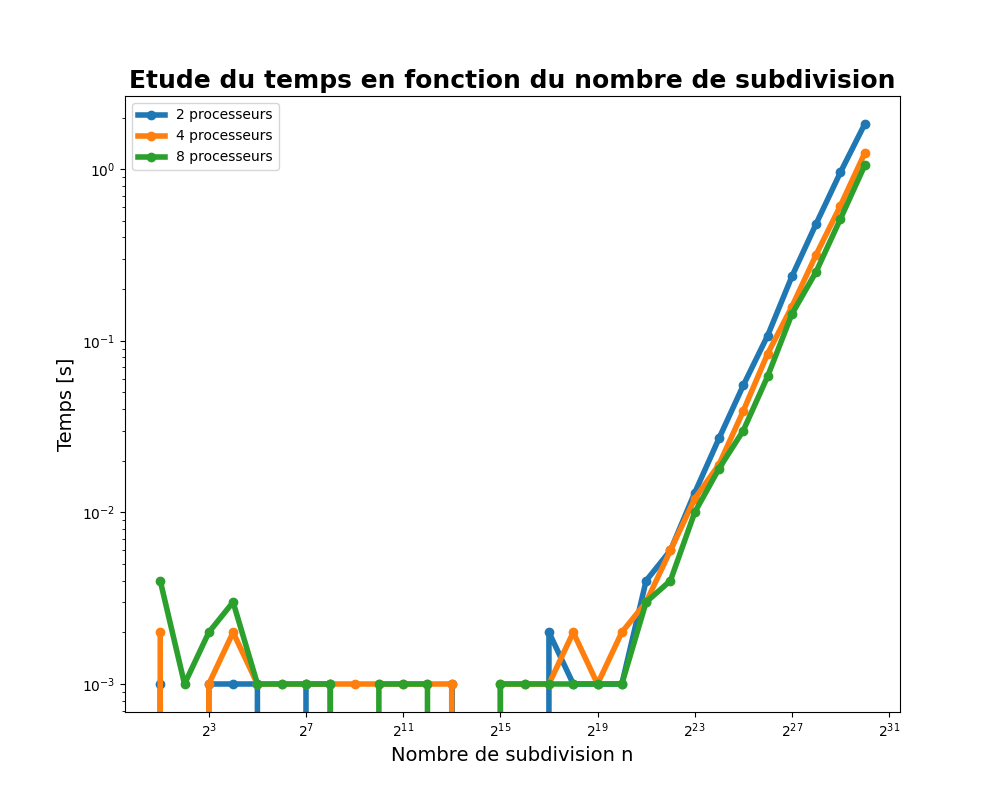
\includegraphics[width=0.45\linewidth]{Images/time_simp_Op_MP.png} &
        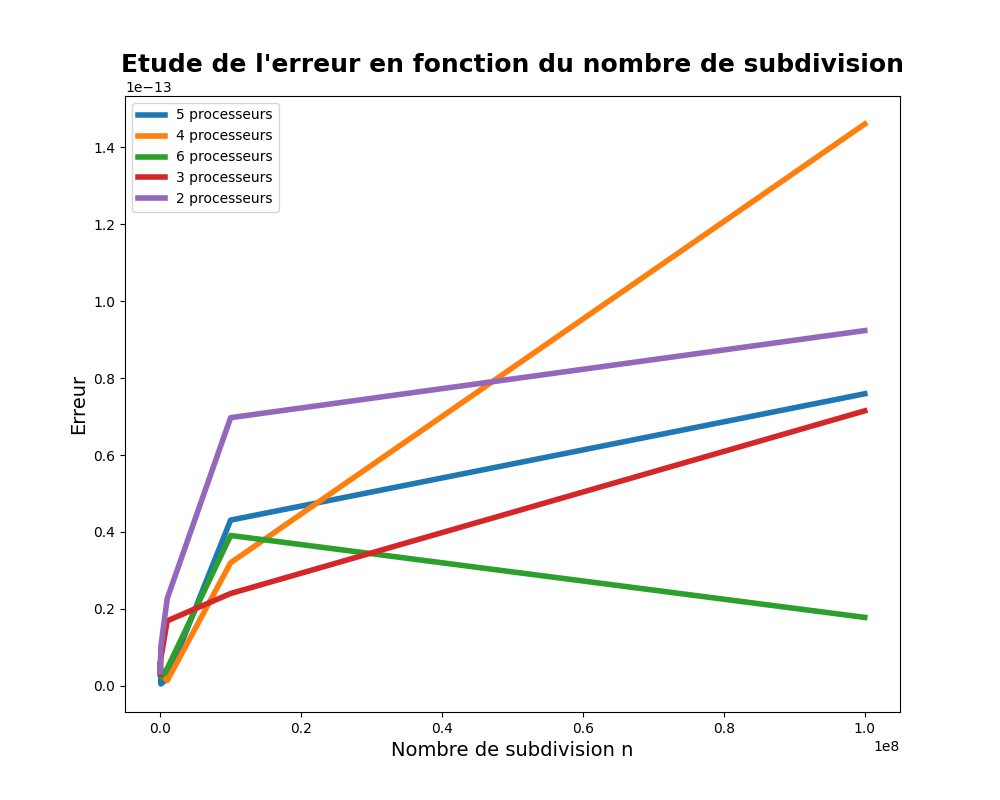
\includegraphics[width=0.45\linewidth]{Images/error_simp_Op_MP.png} \\
        Simpson Temps & Simpson Erreur \\
        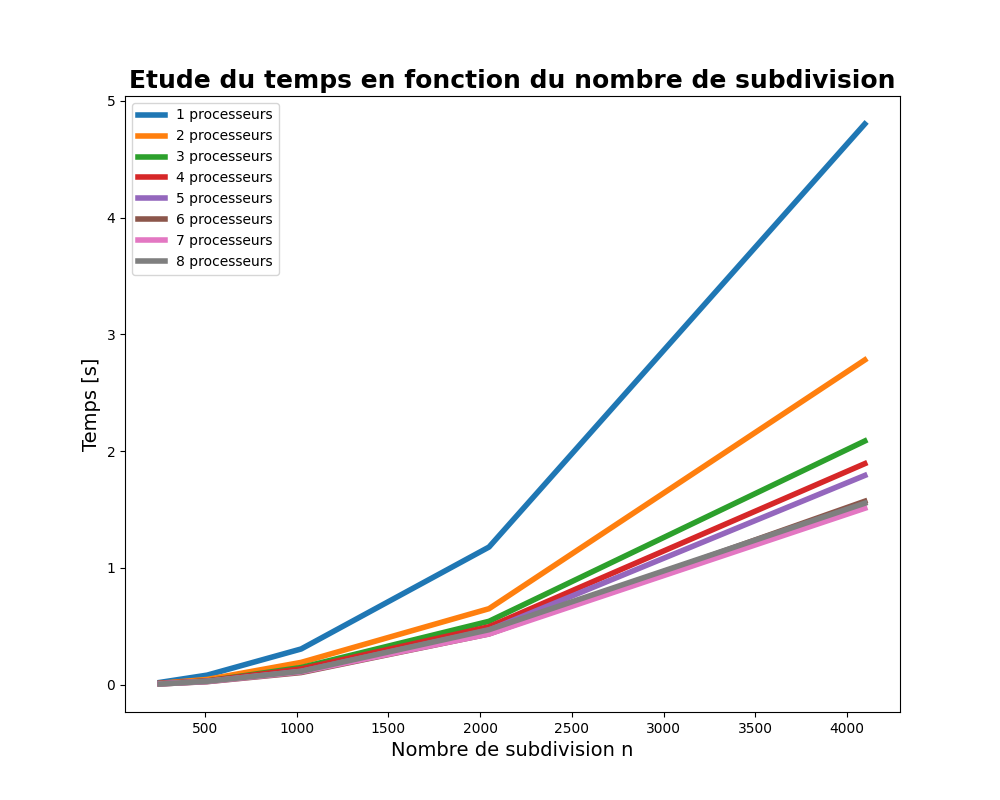
\includegraphics[width=0.45\linewidth]{Images/time_gauss_Op_MP.png} &
        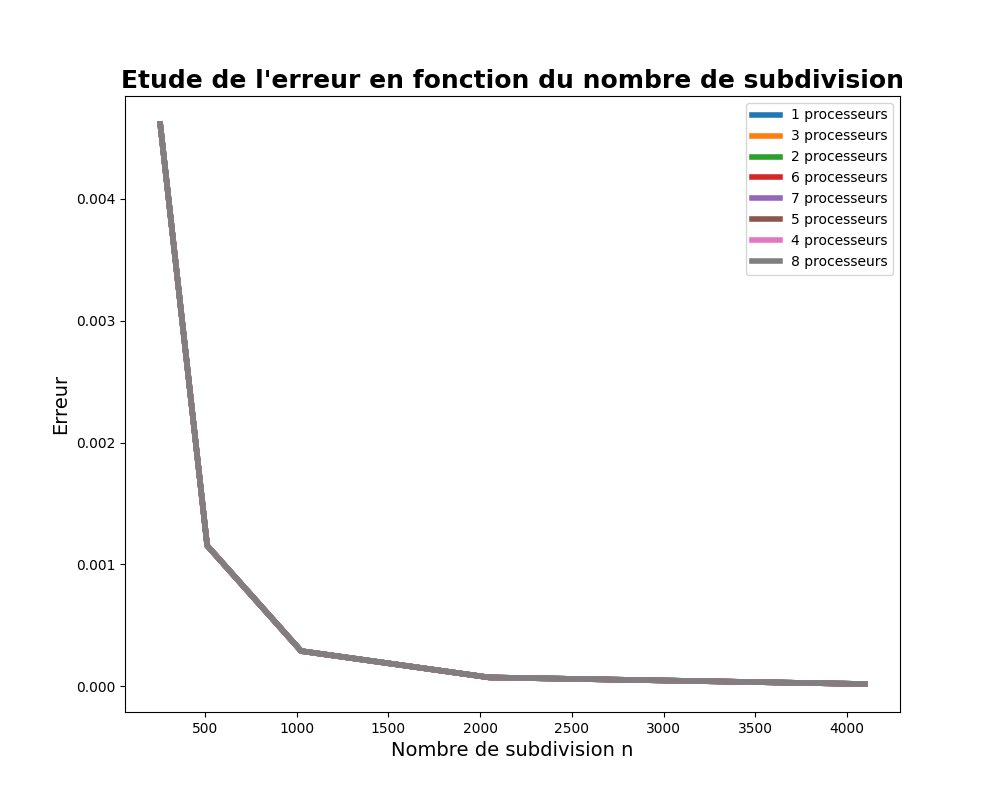
\includegraphics[width=0.45\linewidth]{Images/error_gauss_Op_MP.png} \\
        Gauss 2D Temps & Gauss 2D Erreur \\
    \end{tabular}
        
\end{frame}

\begin{frame}
    \frametitle{OpenMP}
        \small
    \begin{tabular}{cc}
        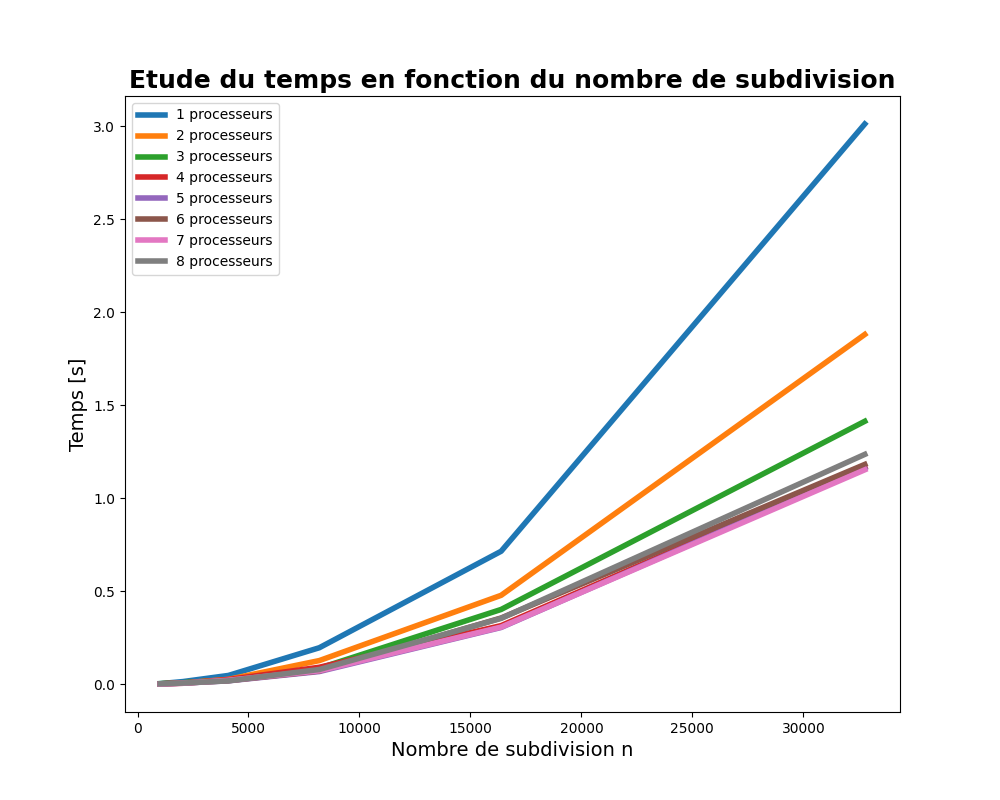
\includegraphics[width=0.45\linewidth]{Images/time_RK_Op_MP.png} &
        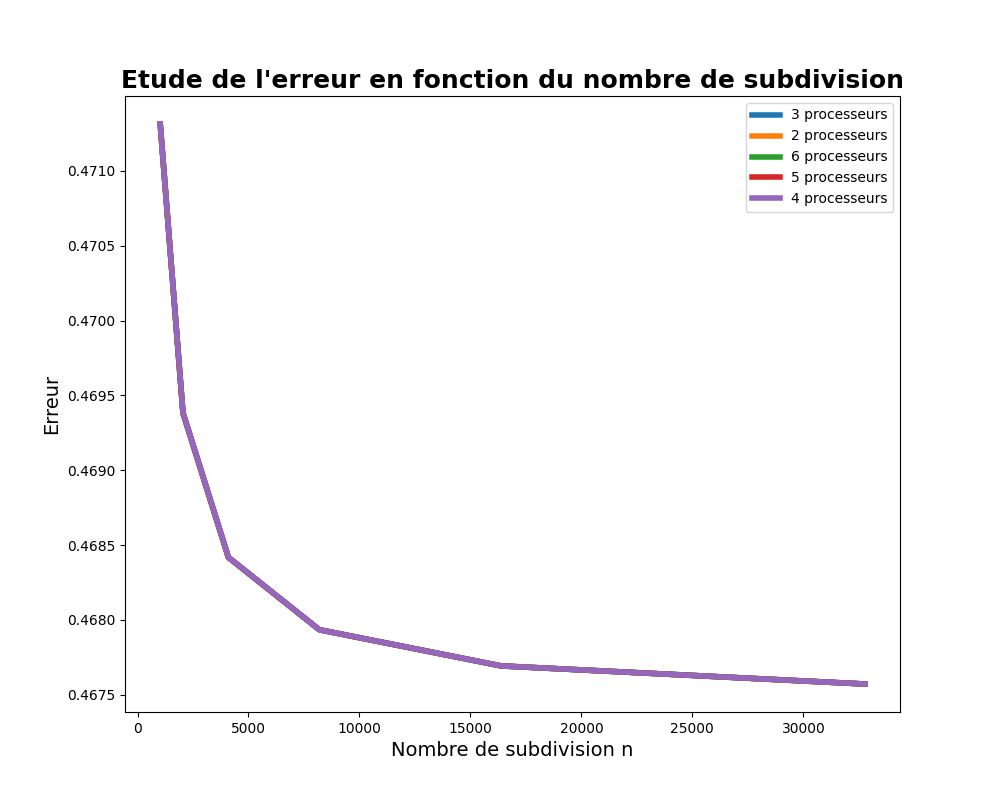
\includegraphics[width=0.45\linewidth]{Images/error_RK_Op_MP.png} \\
        Runge Kutta Temps & Runge Kutta Erreur \\
        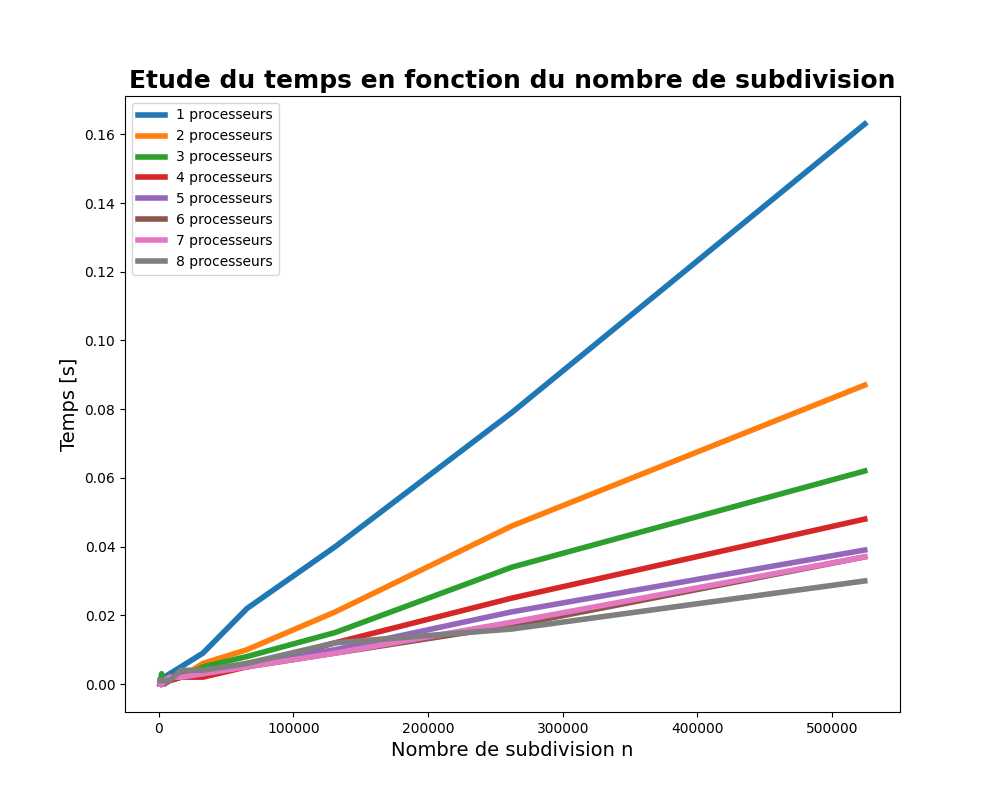
\includegraphics[width=0.45\linewidth]{Images/time_montecarlo_Op_MP.png} &
        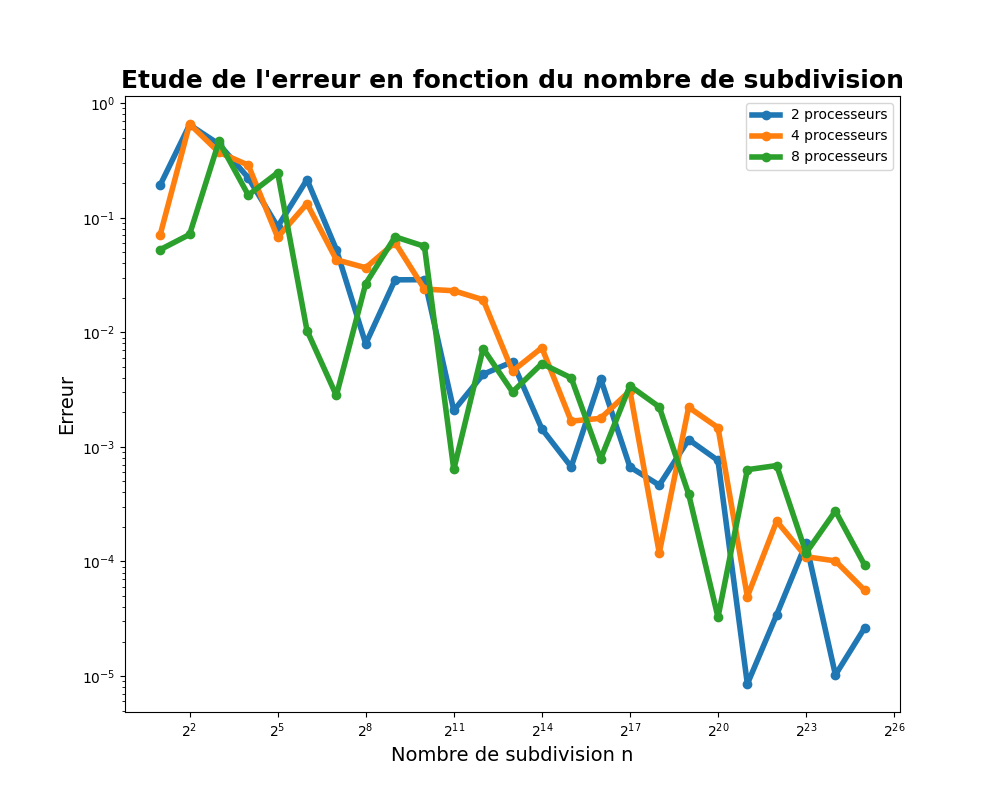
\includegraphics[width=0.45\linewidth]{Images/error_montecarlo_Op_MP.png} \\
        Monte Carlo Temps & Monte Carlo Erreur\\
    \end{tabular}
        
\end{frame}
        
        % \begin{figure}
        %     \begin{minipage}{0.4\linewidth}
        %         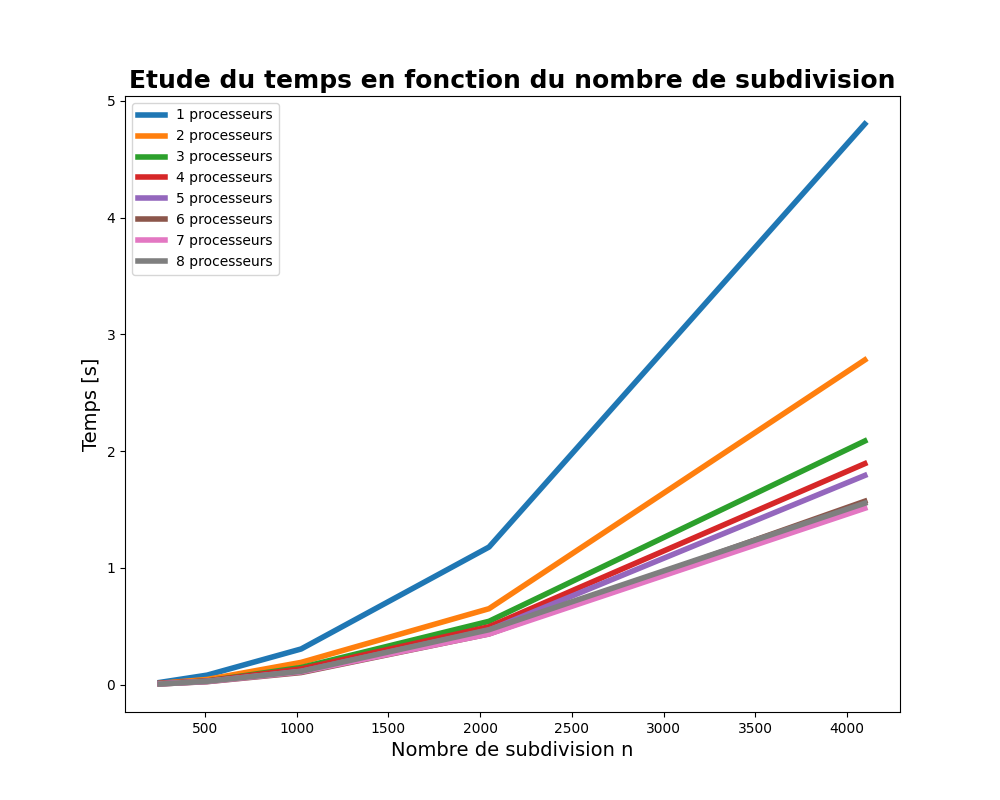
\includegraphics[width=\linewidth]{Images/time_gauss_Op_MP.png}
        %         \caption{Gauss 2D}
        %     \end{minipage}\hfill
        %     \begin{minipage}{0.4\linewidth}
        %         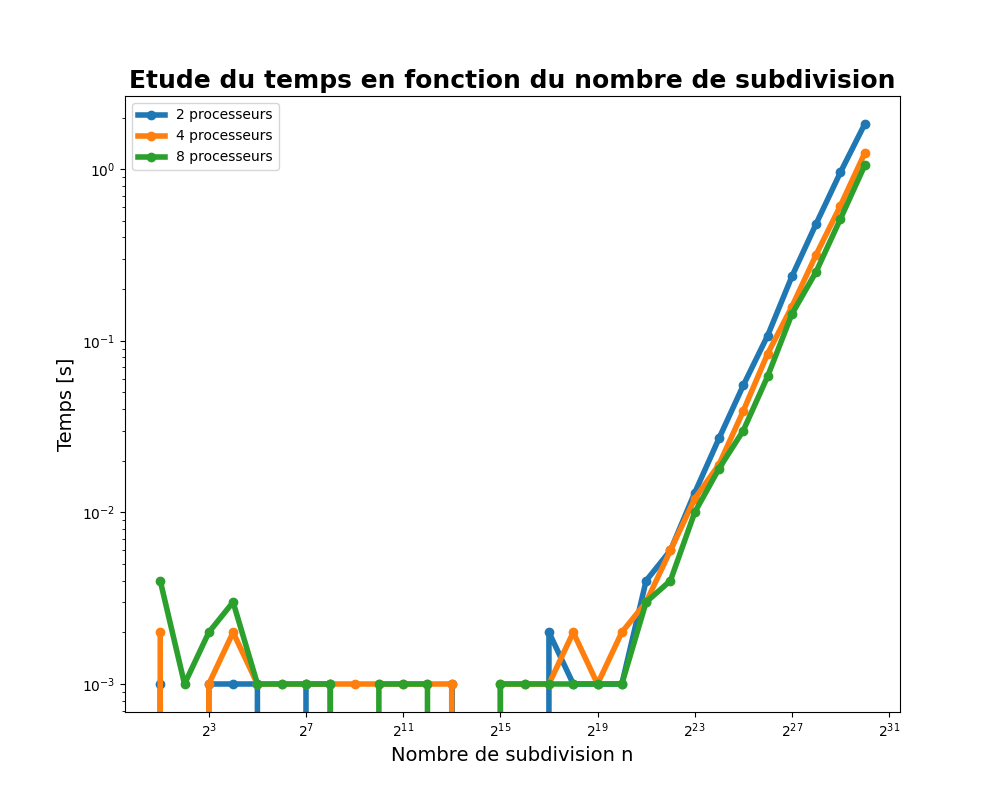
\includegraphics[width=\linewidth]{Images/time_simp_Op_MP.png}
        %         \caption{Simpson}
        %     \end{minipage}
        % \end{figure}
    
        % \begin{figure}
        %     \begin{minipage}{0.4\linewidth}
        %         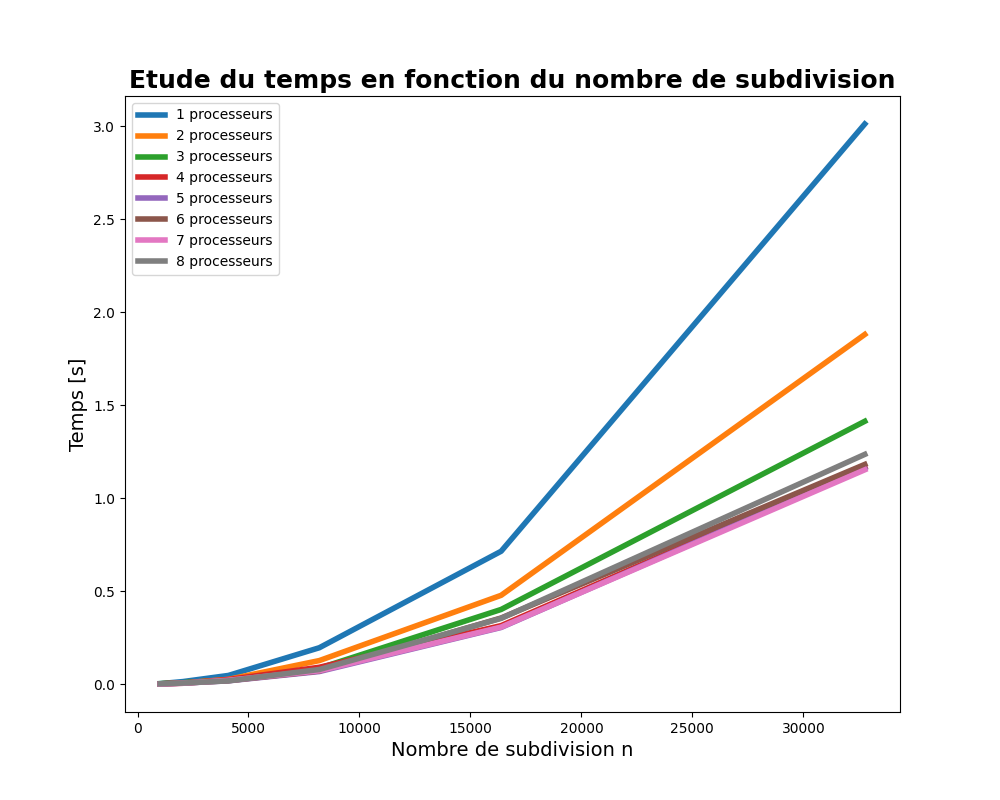
\includegraphics[width=\linewidth]{Images/time_RK_Op_MP.png}
        %         \caption{Runge Kutta}
        %     \end{minipage}\hfill
        %     \begin{minipage}{0.4\linewidth}
        %         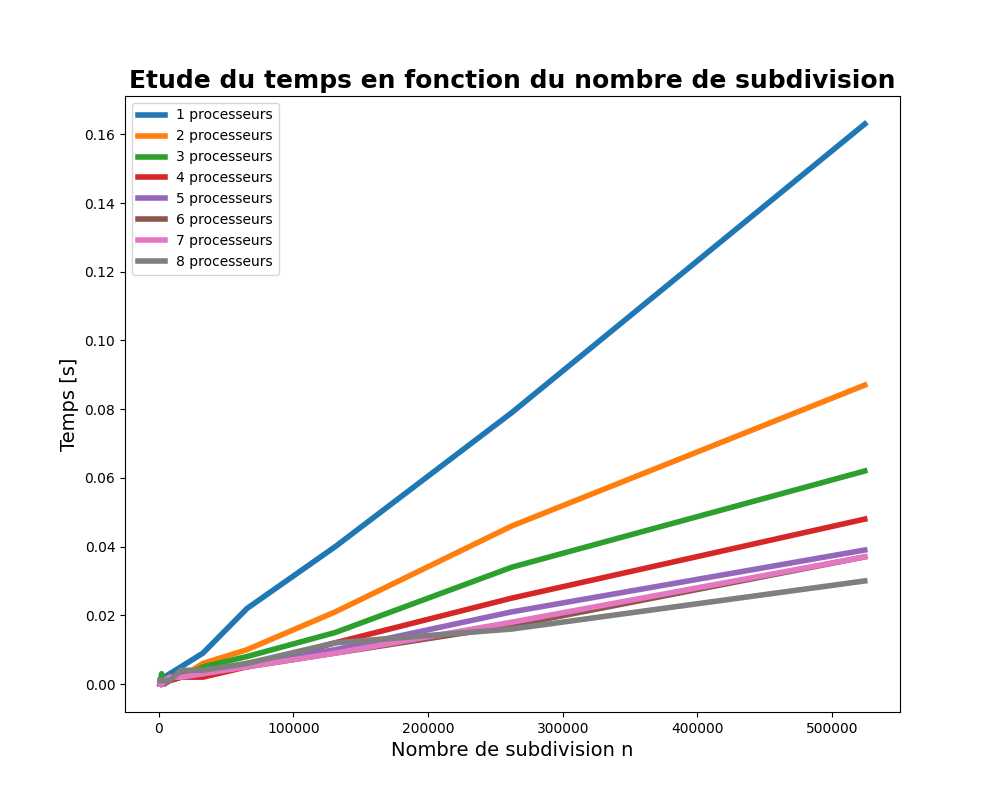
\includegraphics[width=\linewidth]{Images/time_montecarlo_Op_MP.png}
        %         \caption{Monte Carlo}
        %     \end{minipage}
        % \end{figure}

%   \end{frame}


\subsection{MPI}

\begin{frame}
    \frametitle{Résultats pour MPI}
        \small
    \begin{tabular}{cc}
        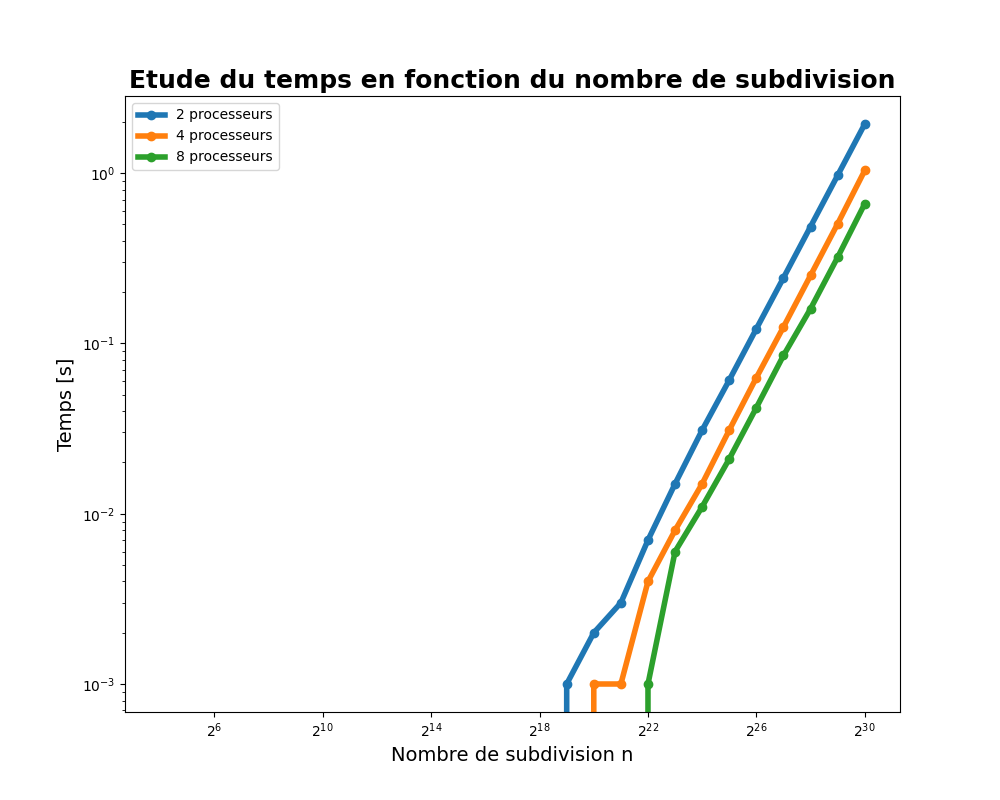
\includegraphics[width=0.45\linewidth]{Images/time_simp_MPI.png} &
        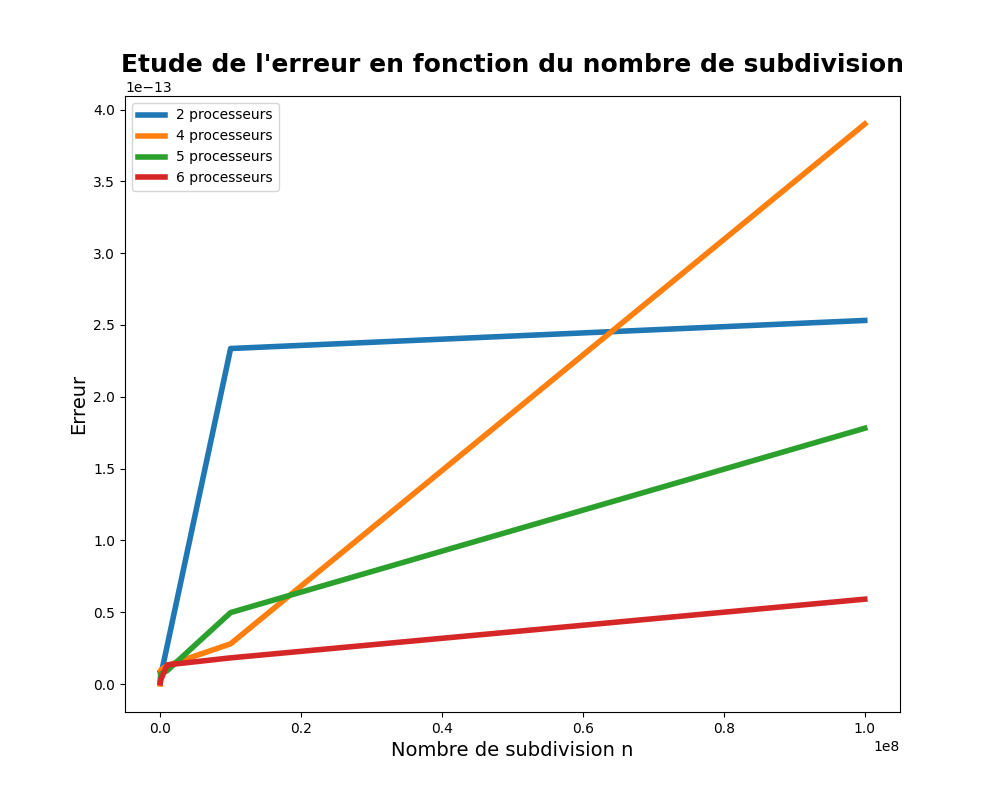
\includegraphics[width=0.45\linewidth]{Images/error_simp_MPI.png} \\
        Simpson Temps & Simpson Erreur \\
        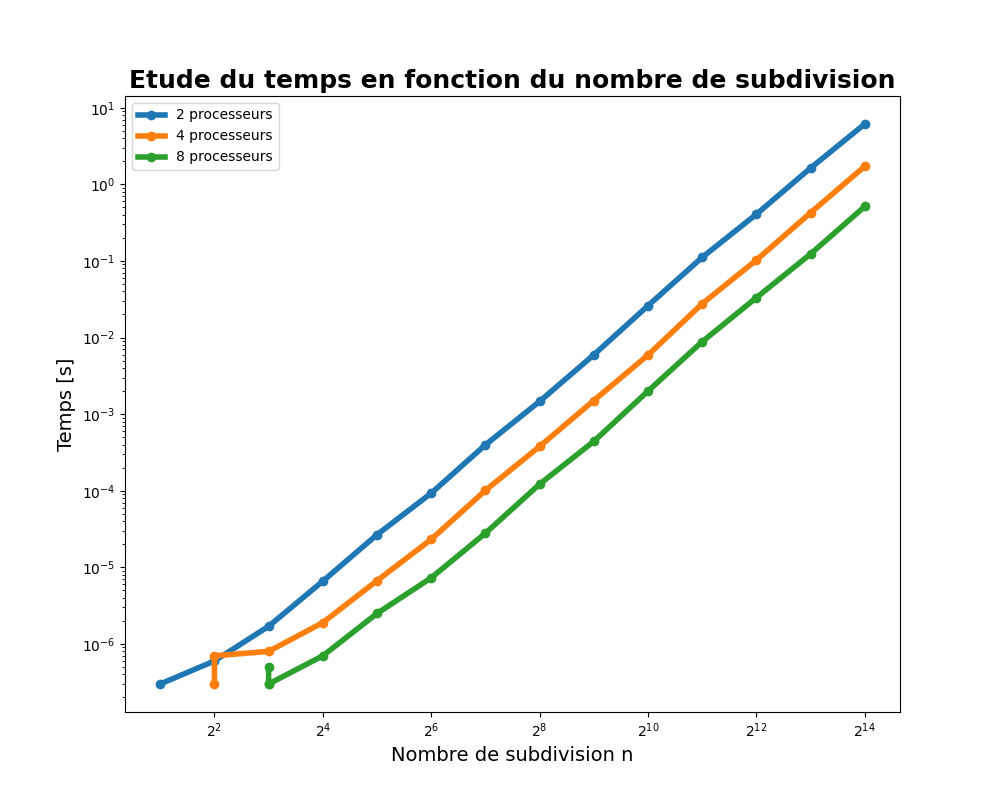
\includegraphics[width=0.45\linewidth]{Images/time_gauss_MPI.png} &
        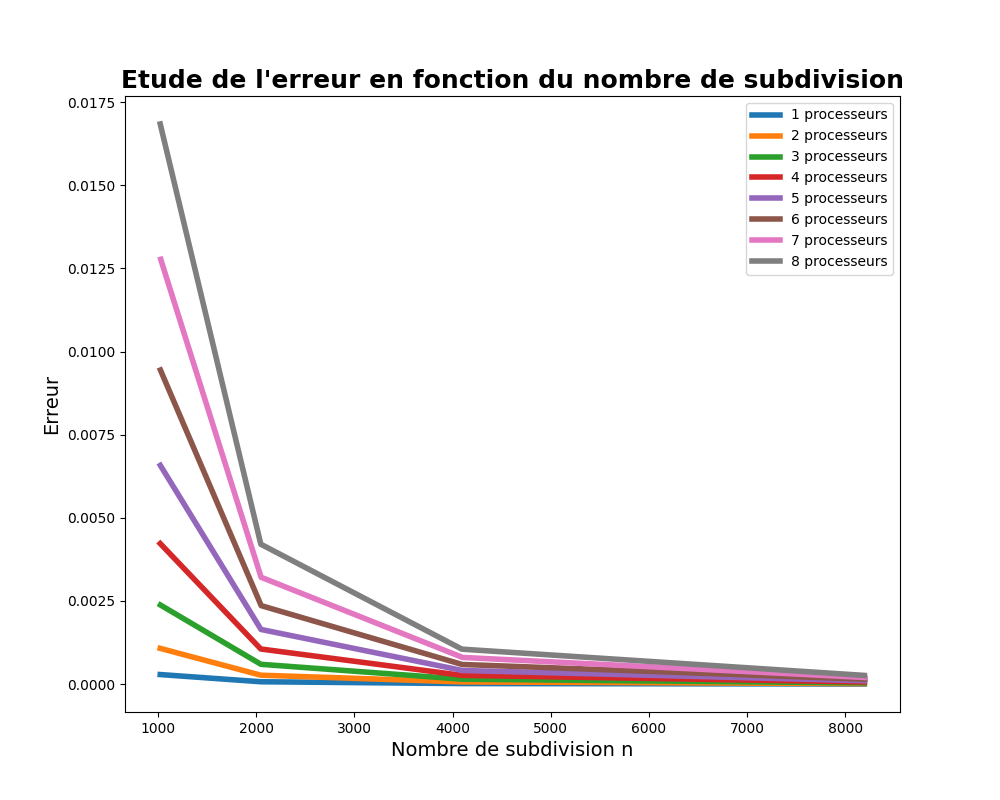
\includegraphics[width=0.45\linewidth]{Images/error_gauss_MPI.png} \\
        Gauss 2D Temps & Gauss 2D Erreur \\
    \end{tabular}
        
\end{frame}

\begin{frame}
    \frametitle{MPI}
        \small
    \begin{tabular}{cc}
        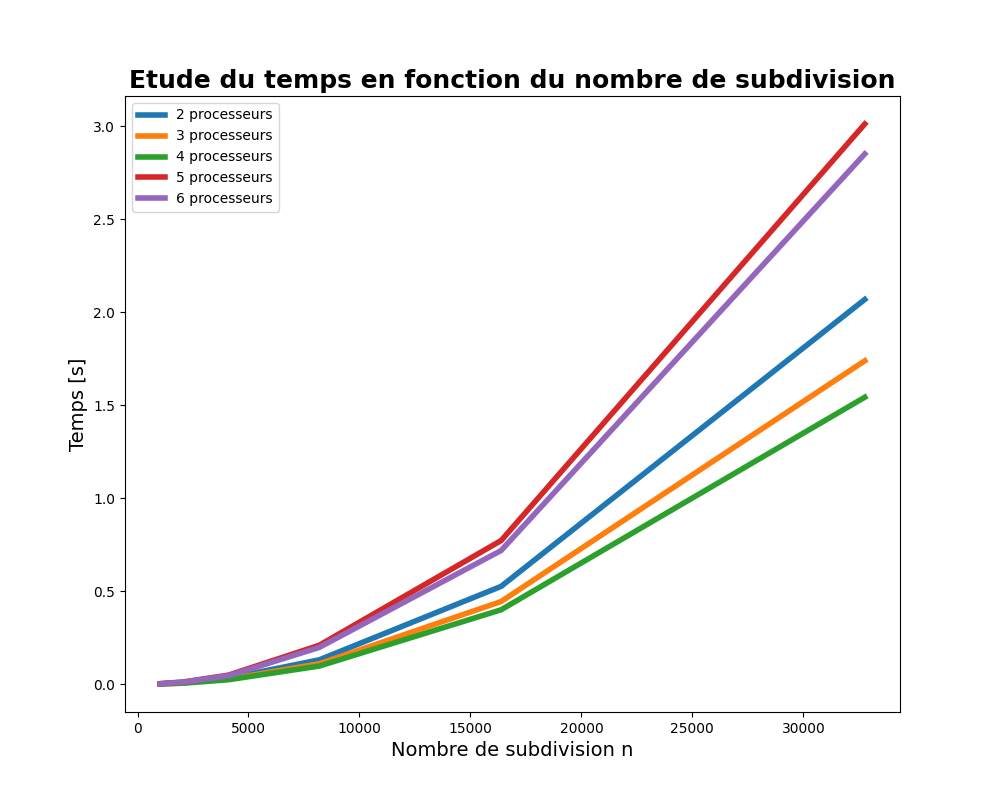
\includegraphics[width=0.45\linewidth]{Images/time_RK_MPI.png} &
        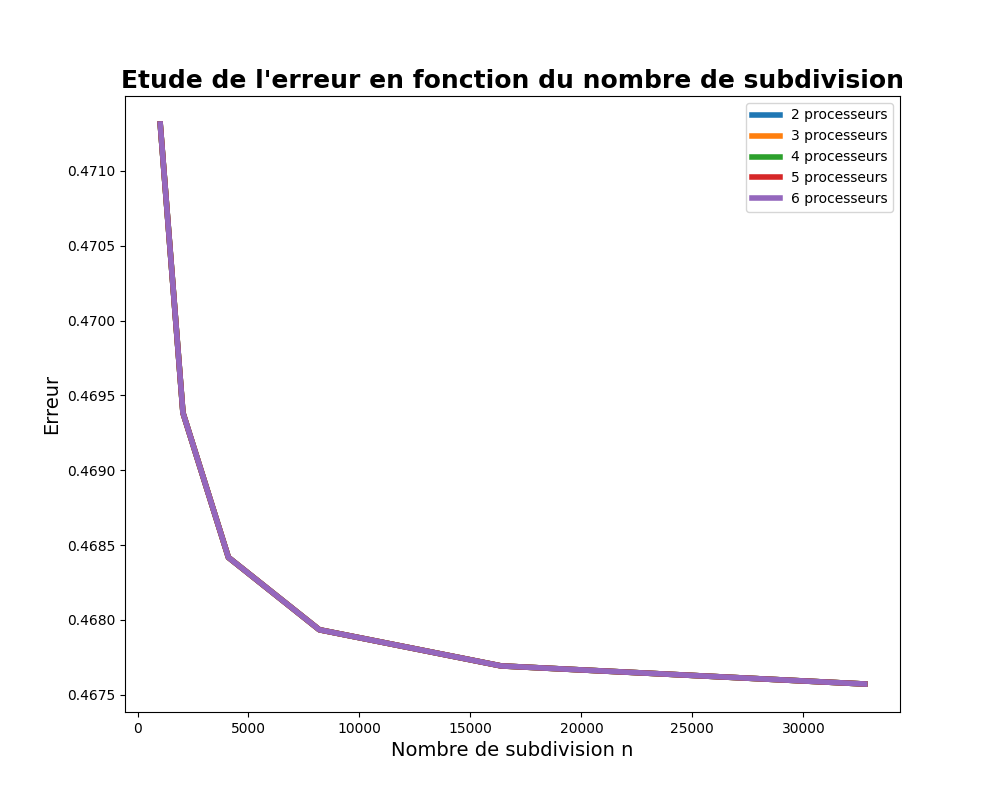
\includegraphics[width=0.45\linewidth]{Images/error_RK_MPI.png} \\
        Runge Kutta Temps & Runge Kutta Erreur \\
        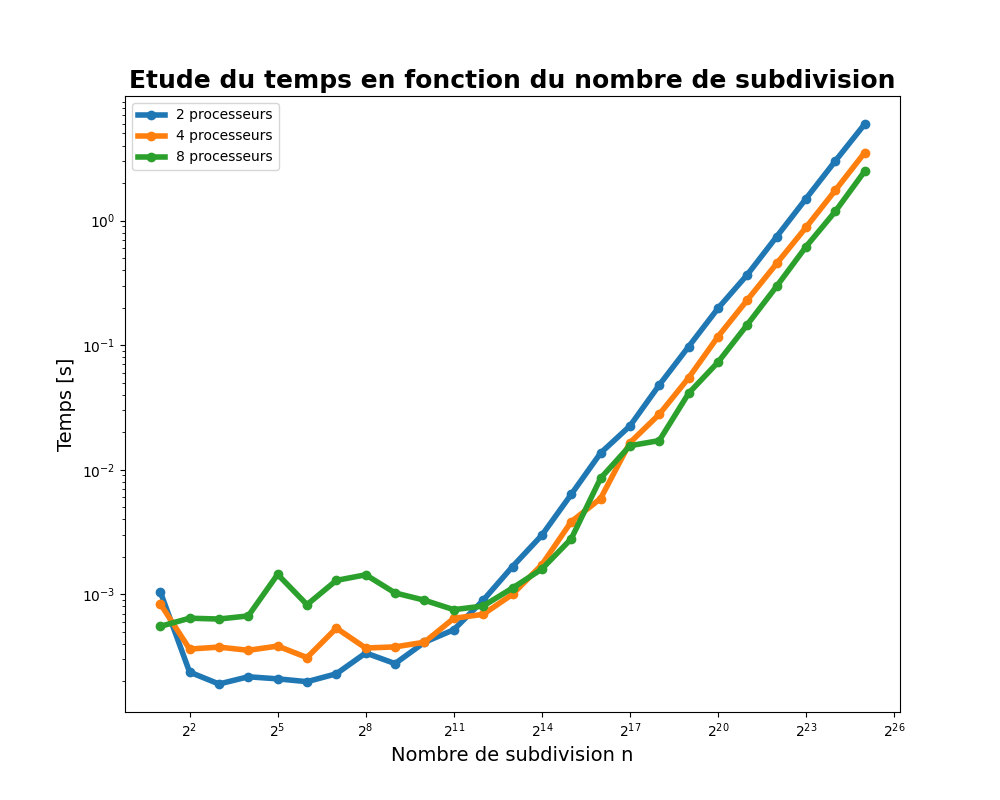
\includegraphics[width=0.45\linewidth]{Images/time_montecarlo_MPI.png} &
        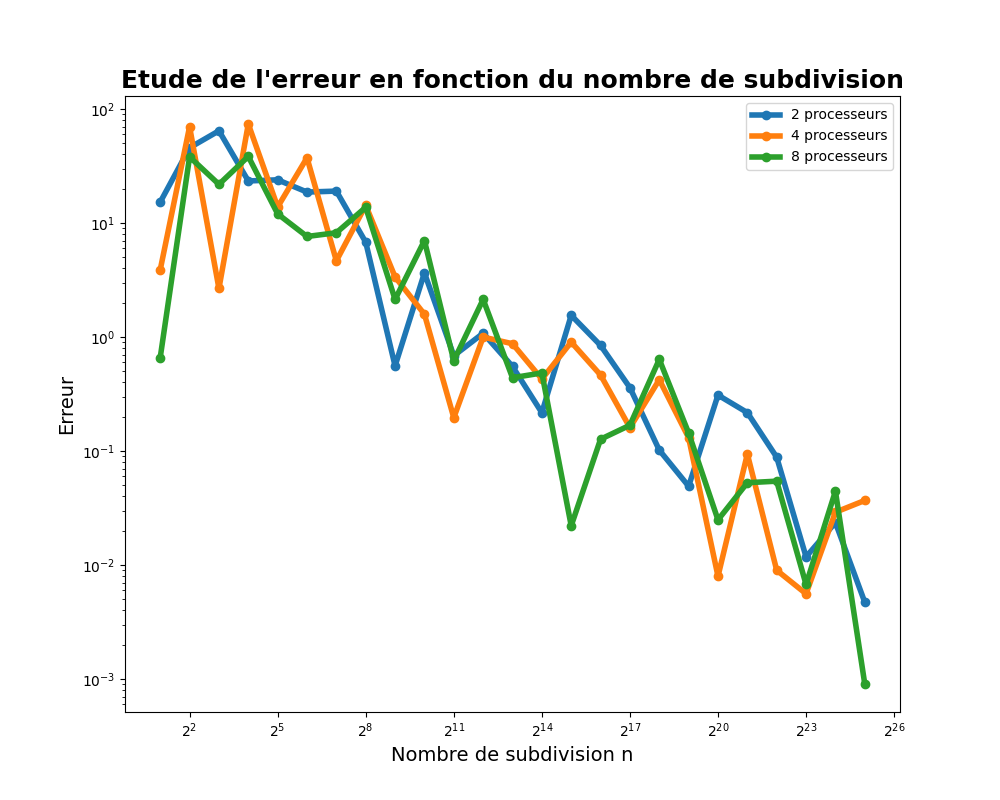
\includegraphics[width=0.45\linewidth]{Images/error_montecarlo_MPI.png} \\
        Monte Carlo Temps & Monte Carlo Erreur\\
    \end{tabular}
        
\end{frame}

\subsection{CUDA}

\begin{frame}
    \frametitle{Résultats pour CUDA}
        \small
    \begin{tabular}{cc}
        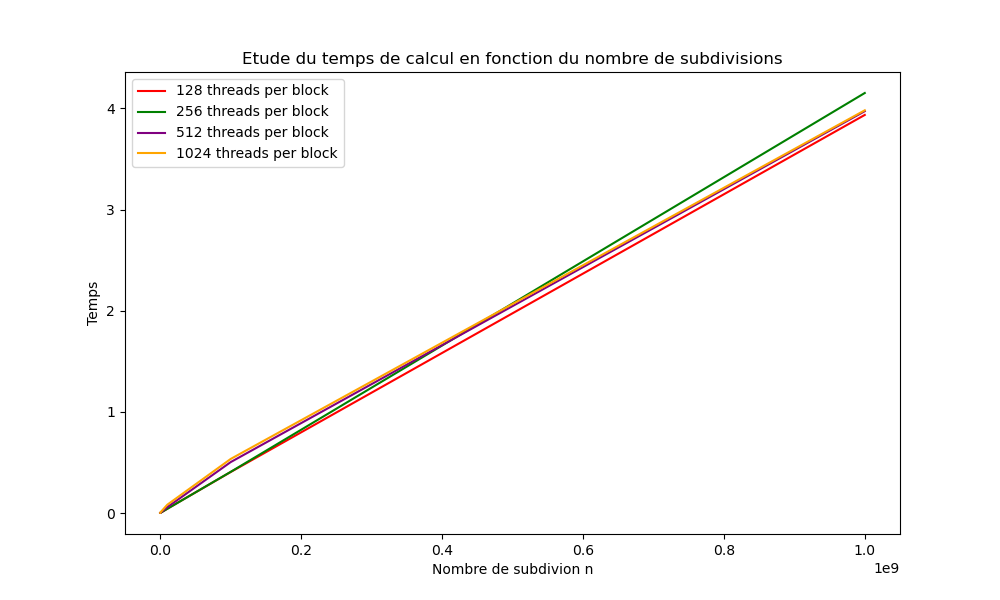
\includegraphics[width=0.45\linewidth]{Images/time_simpson_cuda.png} &
        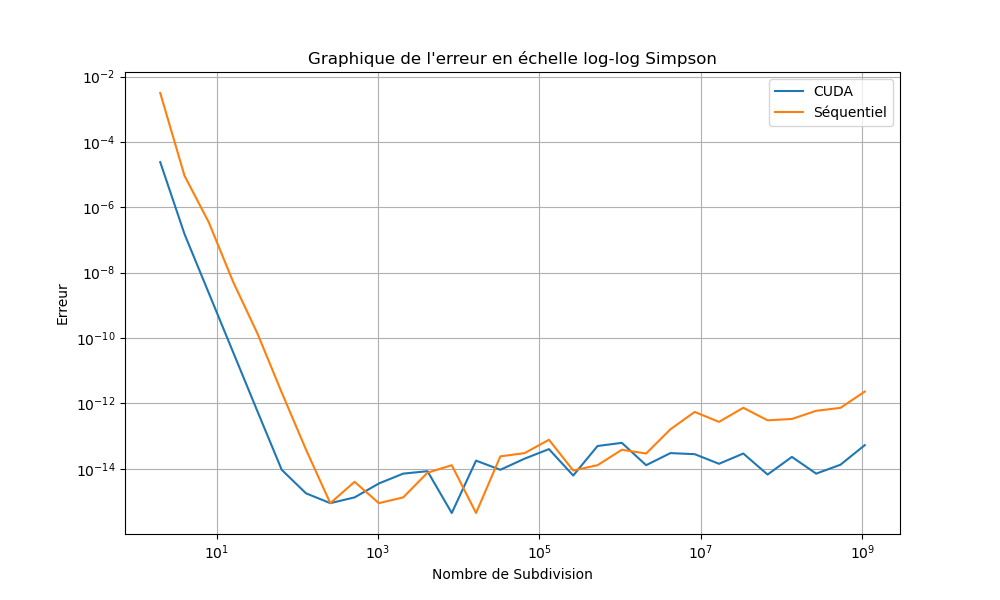
\includegraphics[width=0.45\linewidth]{Images/error_simpson_cuda.png} \\
        Simpson Temps & Simpson Erreur\\
        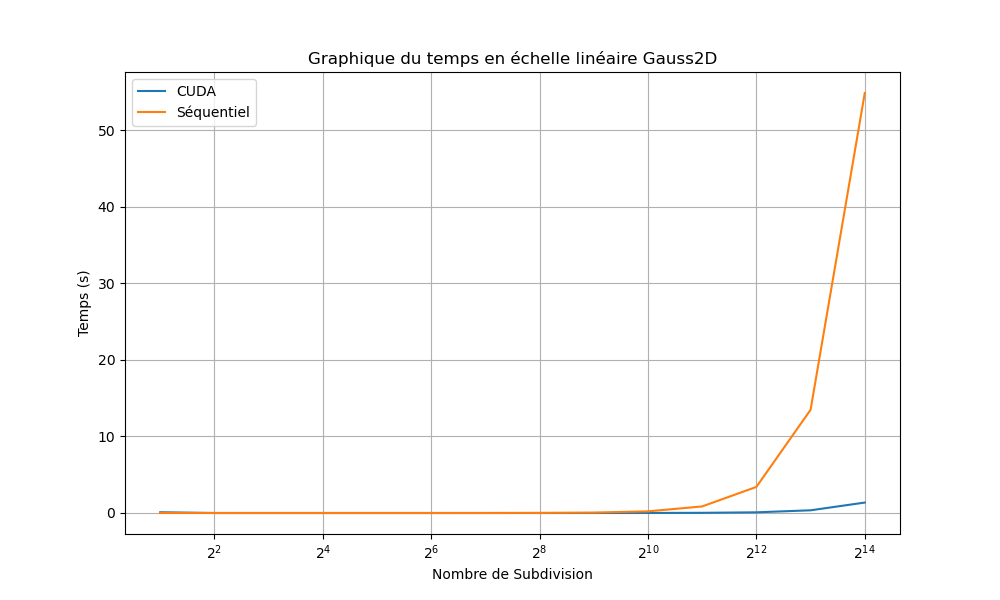
\includegraphics[width=0.45\linewidth]{Images/time_Gauss2D_cuda.png} &
        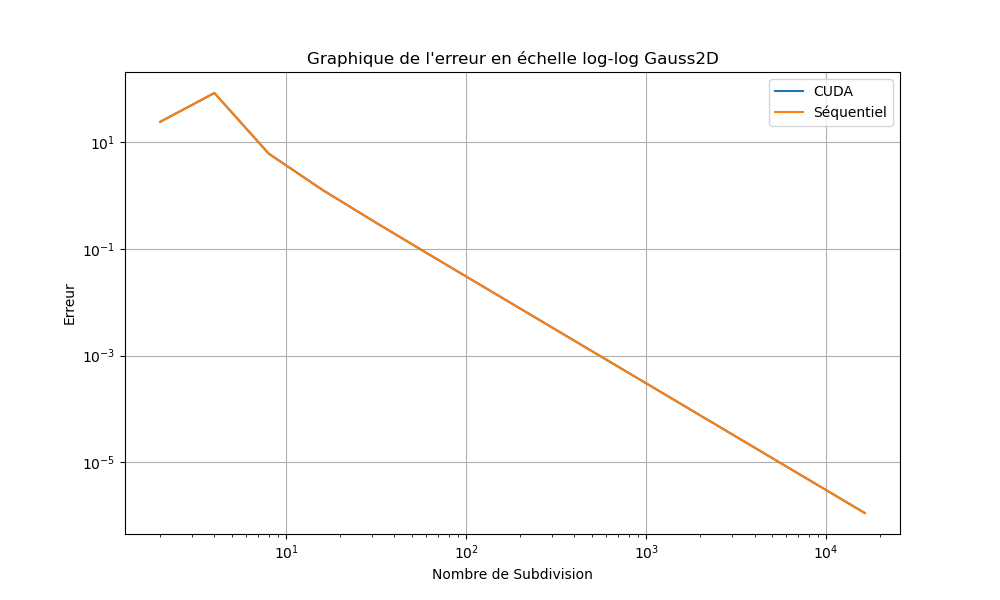
\includegraphics[width=0.45\linewidth]{Images/error_Gauss2D_cuda.png} \\
        Gauss2D Temps & Gauss2D Erreur\\
    \end{tabular}
        
\end{frame}

\begin{frame}
    \frametitle{CUDA}
        \small
    \begin{tabular}{cc}
         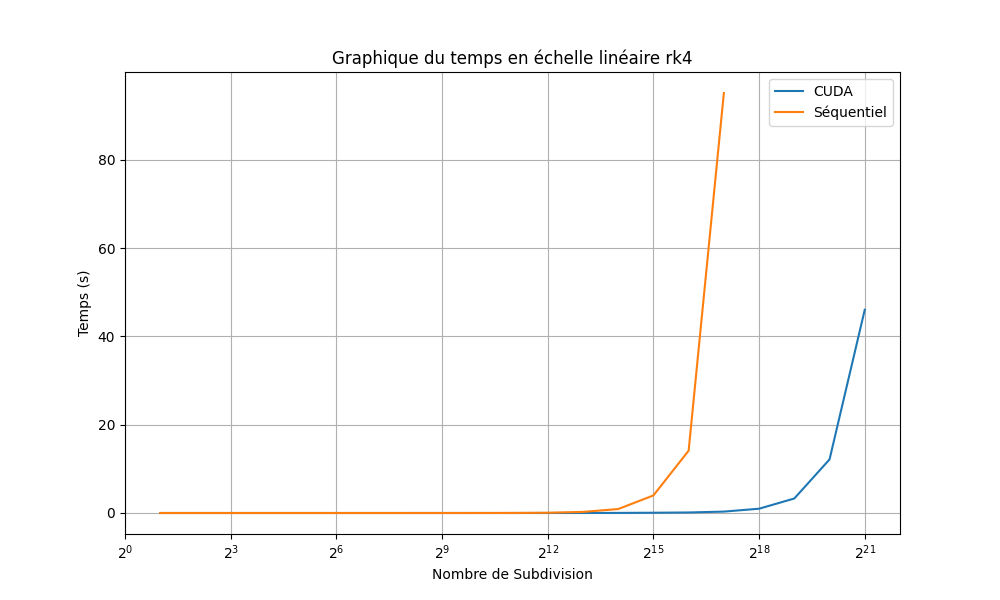
\includegraphics[width=0.45\linewidth]{Images/time_RK_cuda.png} &
         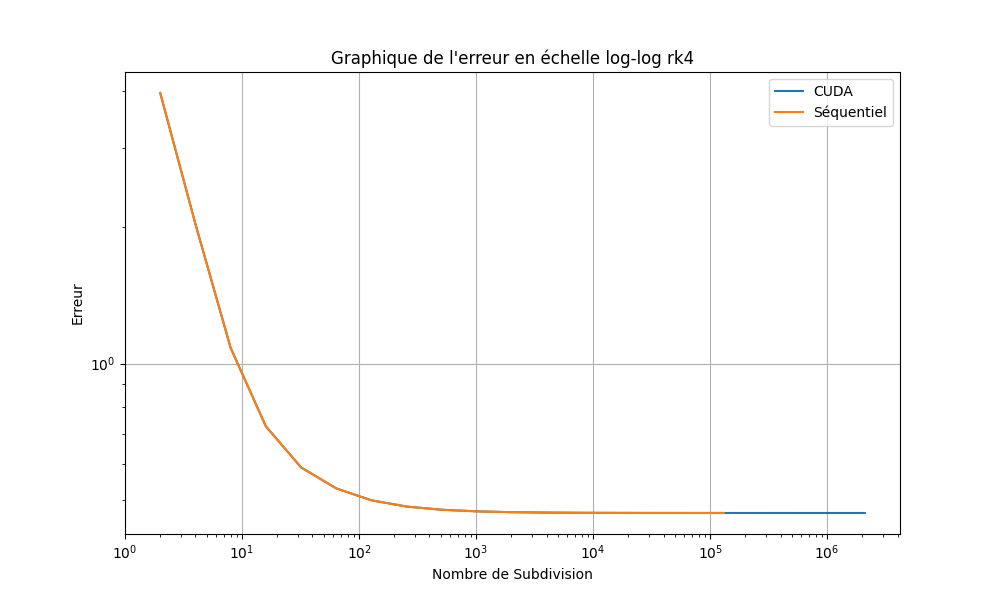
\includegraphics[width=0.45\linewidth]{Images/error_RK_cuda.png} \\
        RK4 Temps & RK4 Erreur\\
         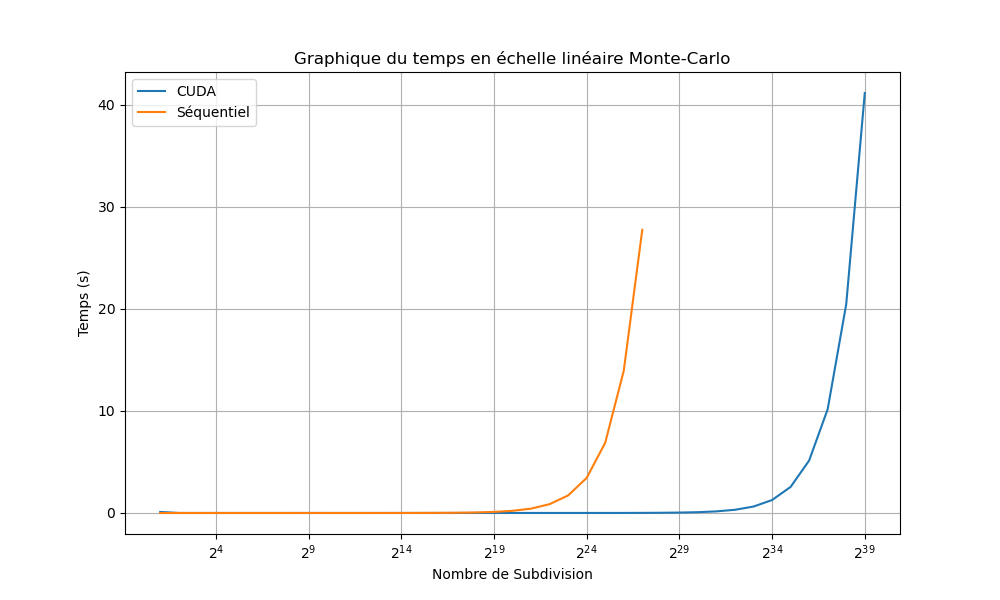
\includegraphics[width=0.45\linewidth]{Images/time_monte_carlo_cuda.png} &
         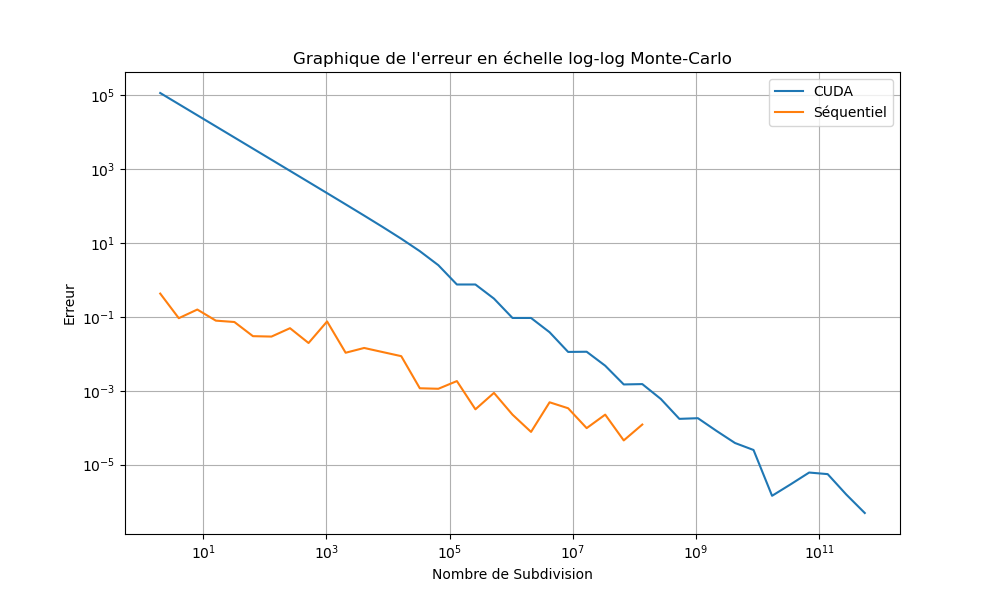
\includegraphics[width=0.45\linewidth]{Images/error_monte_carlo_cuda.png} \\
        Monte Carlo Temps & Monte Carlo Erreur\\
    \end{tabular}
        
\end{frame}


\end{document}